\section{Component overview}

To interact with the physical world, our systems utilizes a stepper motor and
a specialized adapter to perform the tuning on the guitar.
\paragraph{}

\begin{itemize}
    \item We utilize the NEMA 17 stepper motor, commonly used in 3D printers and
    similar eletronic projects, due to its high torque and precsion.
    \item The stepper motor is controlled by a A4988 driver~\cite{A4988}, which allows for microstepping
    and a simplified use of the control signals.
    \item To support the driver a specialized expansion board, shown in Figure~\ref{fig:driver_expansion_board}
    was used,
    which simplified the control connections and power supply.
    \item A custom 3D-printed adapter was designed by taking inspiration from existing designs,
    and is used to connect the stepper motor to the guitar's tuning pegs.
\end{itemize}
\paragraph{}
A raffiguration of the implemented motor control system can be seen in Figure~\ref{fig:system_overview}.

\begin{figure}[htbp]
    \centering
    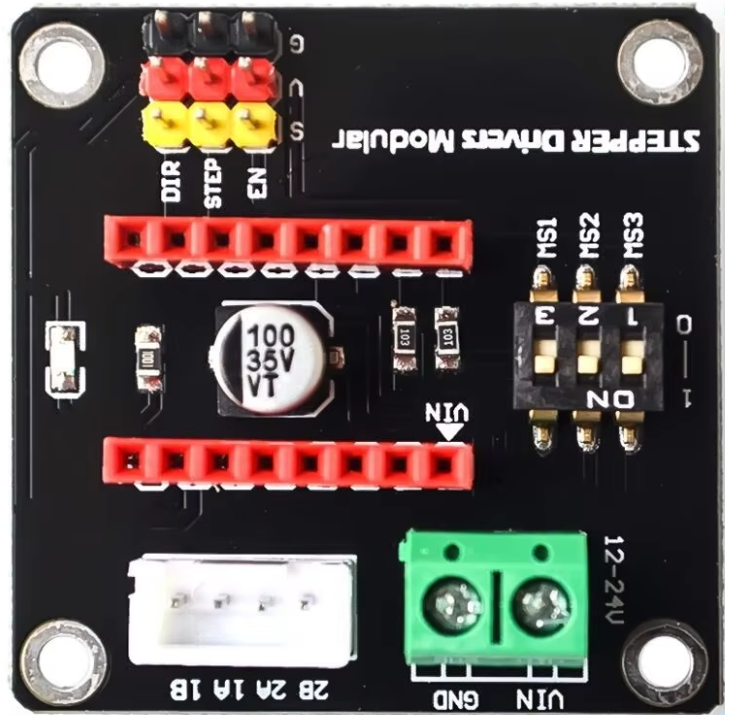
\includegraphics[width=0.5\textwidth]{figures/Driver_expansion_board.png}
    \caption{Driver expansion board}
    \label{fig:driver_expansion_board}
\end{figure}

\begin{figure}[htbp]
    \centering
    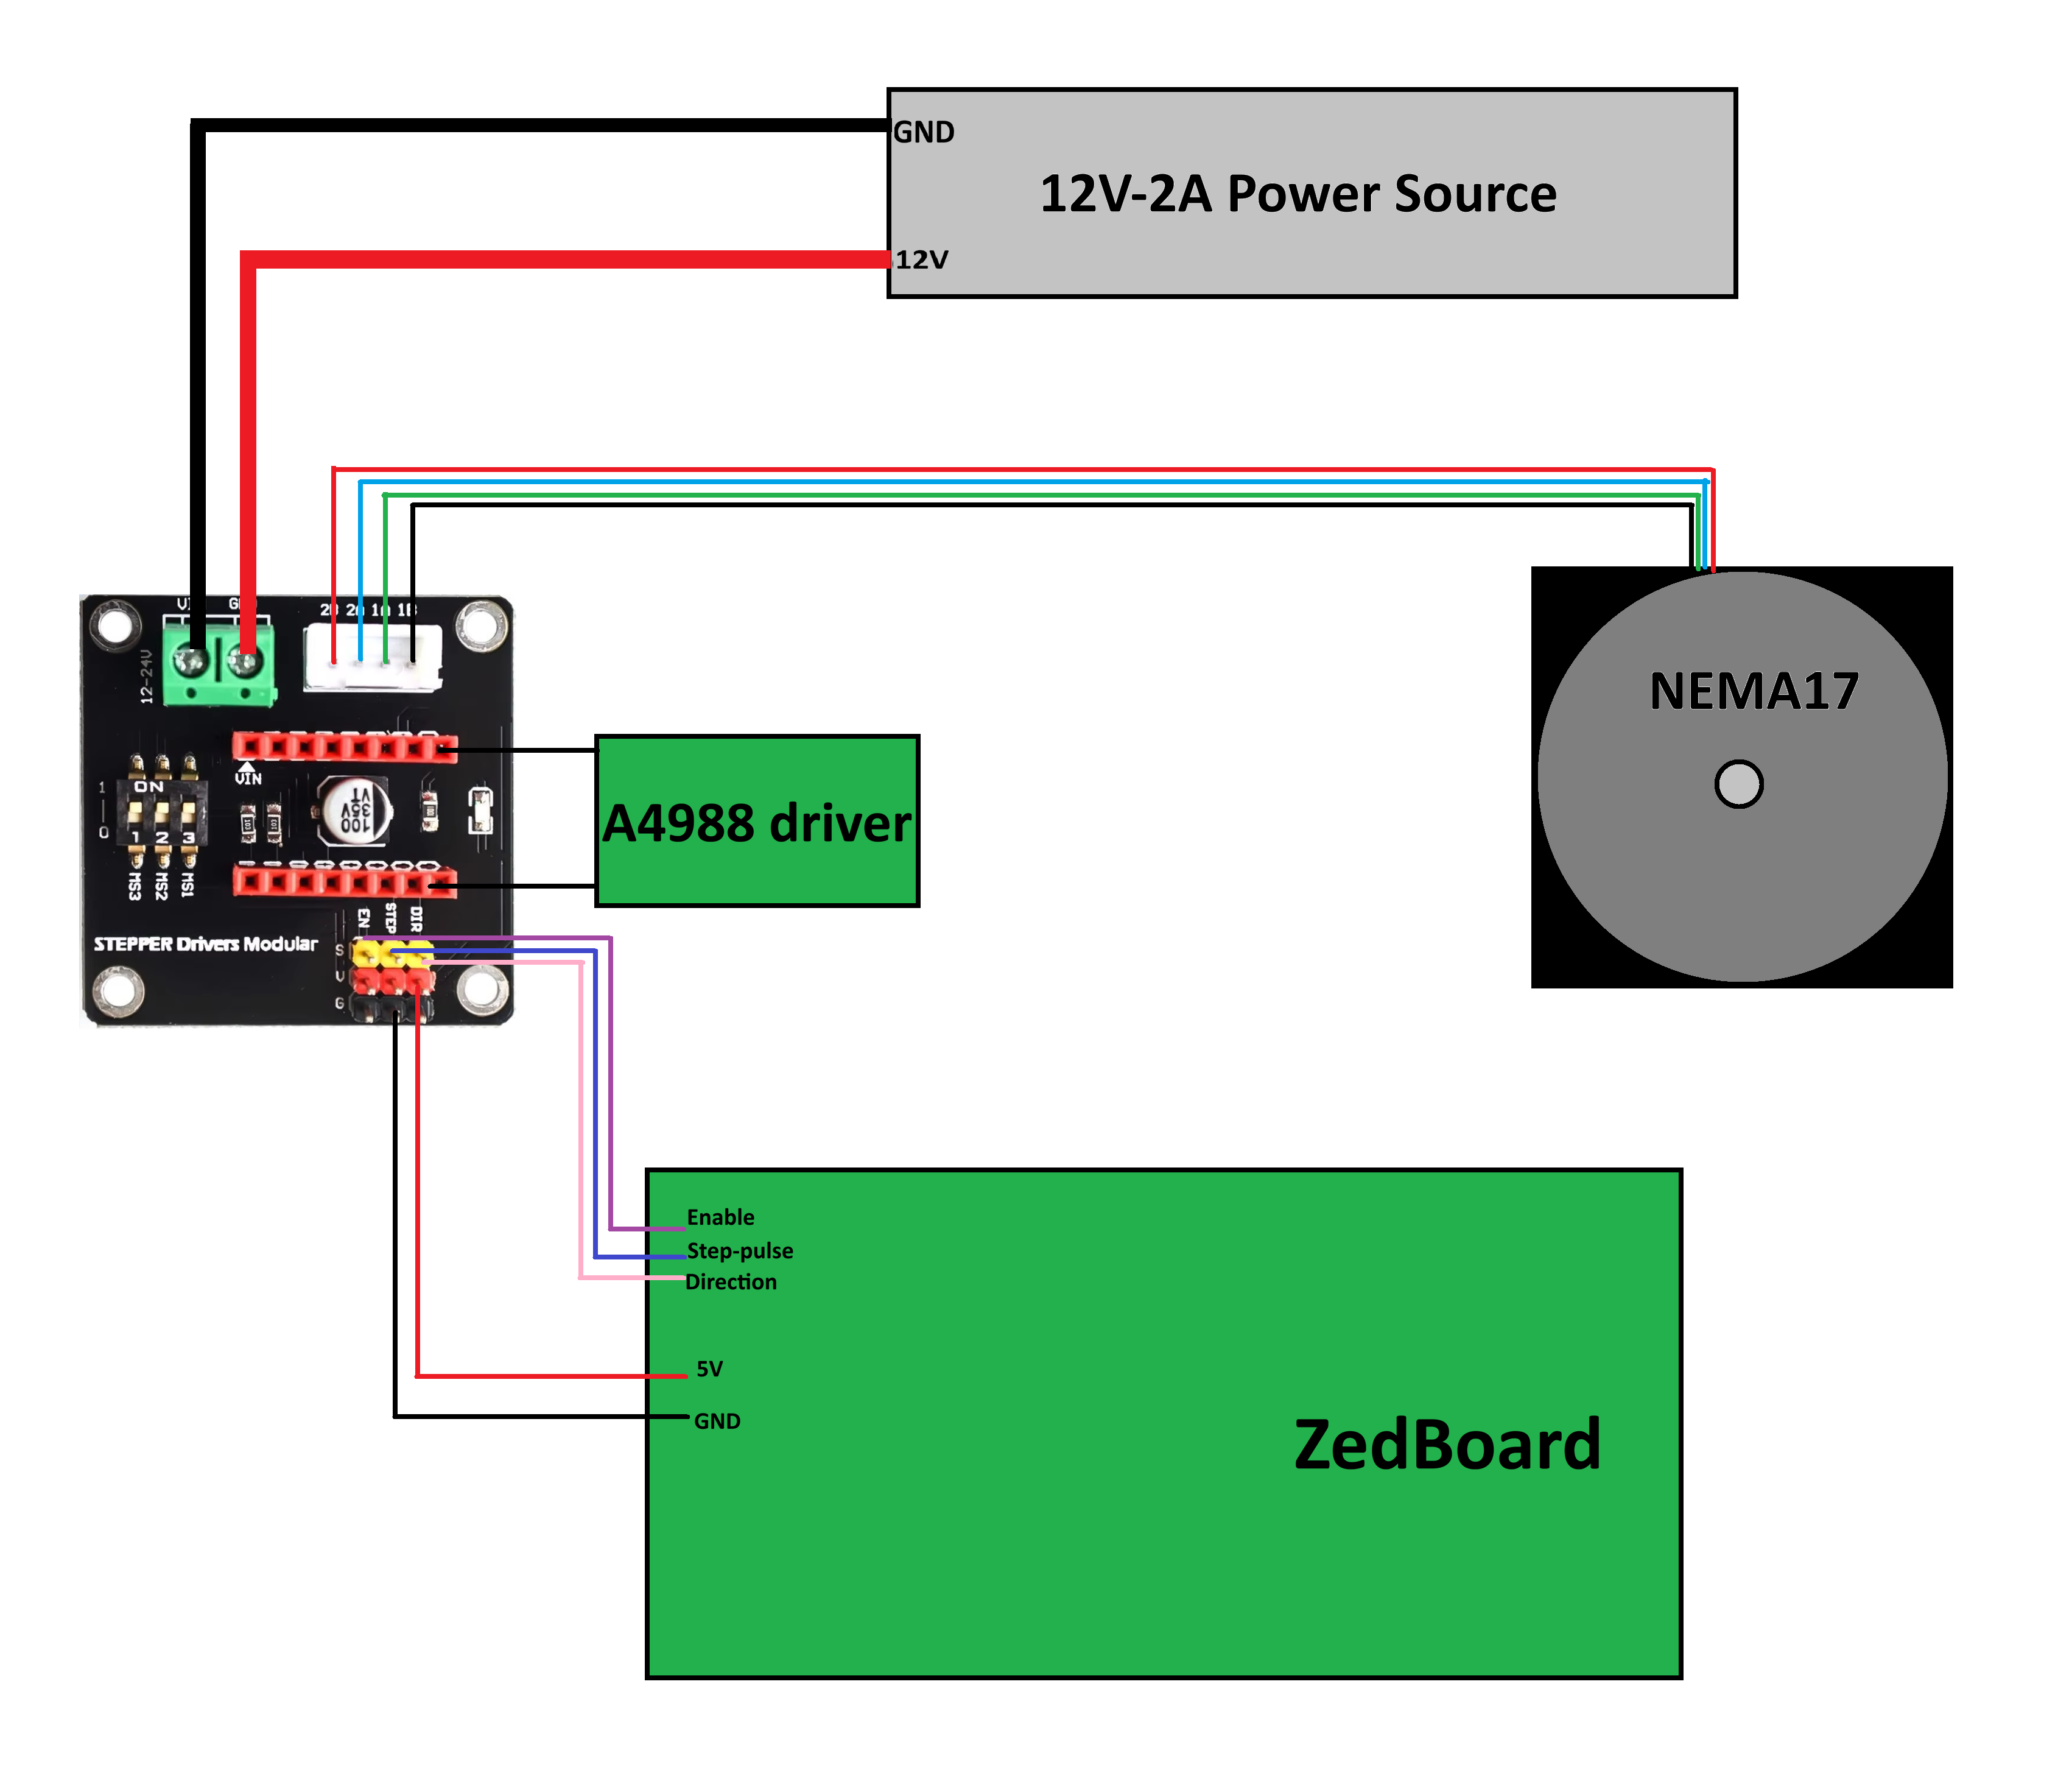
\includegraphics[width=0.5\textwidth]{figures/Motor_system_overview.png}
    \caption{System overview}
    \label{fig:system_overview}
\end{figure}

\section{Control logic}

The stepper motor's control logic is driven by the 100 MHz clock of the ZedBoard,
which is then divided internally inside the dedicated module.
Extensive testing was performed to find the optimal frequency at which we could operate
the motor to unleash enough torque, and for this goal we implemented a switch between 2
different hard-coded frequency divider values, allowing us to perform 2 test with each generation of the Bitstream.
We settled on generating a step-pulse every 2.000.000 clock cycles,
which corresponds to a final frequency of 25 Hz.
\paragraph{}

Other than the clock divider, the control logic also produces the 'direction' and
'enable' signals, which decide the direction of rotation and whether the motor is active or not.
These signals are generated as a result of the comparison between the target frequency and
the current one, receive from the audio processing module.


\section{A4988 driver}

The A4988 driver is a microstepping driver, used to control bipolar stepper motors.
It's commonly used in 3D printers and similar projects, often paired with the NEMA 17.
The driver is controlled by the 3 signals 'step', 'direction' and 'enable',
generated by the control logic module, and is powered by a 5V supply.
\paragraph{}

It allows to drive the stepper motor in smaller steps than its full step size,
resulting in smoother and more precise movements, thanks to the 'microstepping' feature.
With the help of 3 switches on the driver's expansion board, the A4988 can be
configured to divide each full step into 1, 2, 4, 8 or 16 microsteps, trading speed for precision.
To better utilize this functionality, the frequency of the step-pulse is
divided by the chosen microstepping factor, and must be increased accordingly
to maintain the same Rotations Per Minute (RPM) as the full step mode.
\paragraph{}
\textit{The relationship between the step-pulse frequency and the RPM of the motor is given by Equation}
\begin{equation}
    RPM = \frac{f_{step} \cdot 60}{steps\_per\_rev \cdot microstepping\_factor}
    \label{equation:RPM}
\end{equation}
Another advantage of the microstepping is that with the same RPM, the motor will receive more
frequent pulses than in full step mode. This keeps it energized for a longer total amount of time,
which results in a higher torque by avoiding long periods where no current is passing through the coils.
\paragraph{}

The A4988 driver also has a built-in current limiting feature, which with the use of a 
potentiometer screw mounted on the chip allows to set the maximum current
that can flow through the motor coils, preventing damage and overheating.
A thermal shutdown feature is also present, which disables the passing of current if
the temperature exceeds a certain threshold, usually caused by a high current draw or
insufficient cooling.
Because of this features, physical tuning of the system had also to be performed
to find the optimal current limit for the motor.
\paragraph{}

We first measured with a multimeter the resistance put up by the driver, while tuning the
potentiometer, and then we calculated the current limit using
the manufacturer's~\cite{A4988} Equation~\ref{equation:current_limit}.
\begin{equation}
    I_{max} = \frac{V_{ref}}{8 \cdot R_{sense}}
    \label{equation:current_limit}
\end{equation}
Wanting to obtain as much torque as possible, and consequently an higher current limit, we
set the potentiometer to obtain a $V_{ref}$ of 1.07 V.
Considering the fixed $R_{sense}$ of 0.1 $\Omega$ due to the internal resistors
of the A4988, we calculated a current limit of 1.34 A.

\section{NEMA 17 stepper motor}

The NEMA 17 is a bipolar stepper motor. In unipolar motors the current is drawn from
a common connection, and sent to different sides of the coils by switching between the ground connections.
In bipolar ones, the current is sent through the same path inside the coil, and the
\textbf{polarity} must be reversed for each step to happen.
This process requires a more complex circuit, complete of an H-Bridge, which is
implemented inside the A4988 driver.
\paragraph{}

Bipolar stepper motors utilize the totality of the copper coil, which results in a much higher
torque than unipolar motors, but can cause an increase in heat production.
During the first phases of the project we tested the unipolar 28BYJ-48 stepper motor,
a common and cheap solution for electrinic projects, but we quickly realized that
the torque provided was insufficient to perform the tuning of the guitar.
\paragraph{}

The NEMA 17 has a full-step size of 1.8 degrees, taking 200 steps to complete a full rotation,
with a step accuracy of ±0.09 degrees.
It has a rated Phase Inductance of 2.5 mH, a Phase Resistance of 1.5 $\Omega$ and a
Phase Current of 1.5 A, which is the maximum current that can flow through
the coils without causing damage or overheating.
\paragraph{}
The recommended operating voltage is 12 V, but an argument for the use of a 24 V supply
could be made, since an higher voltage would guarantee a faster current rise time,
and consequently an higher torque.
However, this would increase the risk of overheating and would require a more
complex current limiting circuit, like the DRV8825 driver.
